
\section{Second Part : GluonTS}

\subsection{GluonTS historical}

At the time of writing this master thesis, GluonTS is a very recent toolkit, which is coherent with the fact that the deep learning forecasting field is early itself.
It first release version (\textit{v0.1.0}) is dated from March 3rd 2019.
The implementation of the code has been performed on the version \textit{v0.4.2} released on
November 26th 2019 and as been updated for version \textit{v0.5.0}, released on May 12nd 2020.
These versions are/was still considered as beta versions. This implied several bugs and implementation issues. In particular some models (for example an implementation of the \textit{DeepState} model \cite{deepstate_paper})  failed to run correctly, and the run of "custom" models (implemented using the provided model template) is incompatible with the hybridization functionality, which provides important time optimization, because of a bug. 
And some functionalities that would be useful are not currently implemented, as alternative loss functions (see \ref{custom_loss} section).

\subsection{GluonTS Functioning}

The GluonTS toolkit defines a dataset structure, containing in particular the time series. This dataset, is given to a GluonTS model (pre-implemented or implemented using the provided model template), which use the dataset information (to train and test the model). When the model is evaluated, it gives in all cases as output a distribution for each of the testing time steps, for each time series (see \ref{problem_statement}).
The type of output distribution is defined by the user and discussed in section \ref{distribution}. Concretely, the output information is a set of randomly drawn sample of the predicted distribution,
not the distributions parameters themselves.
The model, if belongs to deep learning models category, must be trained before evaluation, using the chosen loss function (see section \ref{loss}).
The resulting output distributions can be evaluated using the appropriate metrics (see section \ref{metrics}).

\subsection{Datasets} \label{datasets}

GluonTS interface imposes a certain structure of datasets, object used for training and testing  models. There are composed of some mandatory and some optional components.
$`dataset.train`$ is an iterable collection of data entries used for training. Each entry corresponds to one time series.  $'dataset.test$ is an iterable collection of data entries used for inference. $`dataset.metadata`$ contains metadata of the dataset such as the frequency of the time series, the context length,  the prediction length.
%associated features. These associated features are data given in addition to the time series, that will also been seen as input by the network. They can be static, dynamic, real, categorical , etc.

%We should emphasize here that a single moded is trained over all the time series contained in the training dataset . This results in a global model, suitable for prediction for all the time series in the testing dataset as it is defined in the classical way and possibly for other unseen related time series.

GluonTS is optimized to handle multiple time series in parallel. The training time will be significantly increased if the dataset is composed of only one time series of very long length compared to a dataset composed of multiples time series of smaller length. 

As mentioned in section \ref{problem_statement}, in general the training and testing set is composed of the same time series.
The definition of the task whereabouts this master thesis is dedicated, the forecasting of wind turbines production, is not compatible with this general affirmation.
In fact, the goal is to forecast the production of an energy generator using a model which couldn't be trained on the current generator production history, but on others generator production history.
It is nowadays useful to test different configurations of training/testing data, including where the training data and testing data comes from the same generator(s) history. This allow us to test how the forecast quality is influenced by the variation of configuration of input data.

Input data provided by "Blacklight Analytics" is composed of different (raw) time series :

\begin{itemize}
    \item A continuous 6 months history of a wind turbine production , in kWh \newline
    (\textit{6months-minutes.csv})
    \item An history of a wind turbine production, in negative MWh \newline 
    (\textit{mesure\_p\_gestamp.csv})
    \item A 2 days history of two wind turbines production, in negative MWh \newline
    (\textit{2eol\_measurements.csv})
\end{itemize}

All the data is at a frequency of 1 minute, and is converted in positive MWh. 
Nowadays the configuration, because of the GluonTS behaviour optimized to handle multiple time series, these original times series are manually splitted before putting them in dataset structure.
Each time series is manually splitted in certain number of time series of same size. This size is considered as a hyper parameter of the problem ($data\_size$). 

The configurations considered are the following :

\begin{itemize}
    \item All the disposable times series are used as training and testing data. It is referred as "Config A"
    \item \textit{2eol\_measurements.csv} time series used as testing data and the other time series as training data. It is referred as "Config B".
\end{itemize}

GluonTS allow the use of "features", i.e. information used as input to the models additionally to time series information. Not all the models are compatible with this functionality. 
In our case, the different sources of information could be identified using static categorical features. For example, in the configuration A, splitted time series coming from time series \textit{6months-minutes.csv} will have a categorical value of 0, time series from \textit{mesure\_p\_gestamp.csv} the value of 1, times series from \textit{2eol\_measurements.csv} values of 2 and 3. This functionality useful if the different sources have significant differences.

The size of the prediction window  \textit{BlackLight Analytics} is interested in is 10 minutes, i.e a predict length of 10  for a frequency of 1 minute. The context length, as defined in section \ref{problem_statement} is a hyper parameter of the problem indicating the number of time steps considered as input for the model network.



\subsection{Quantiles} \label{goal}

GluonTS allow selecting the values of quantiles that will be computed, to evaluate the metrics and to possibly use these information in loss function.
This functionality is used in section \ref{custom_loss}.
%In the current implementation, the value of $e$ is $1\%$, the security quantile is $quantile(0.99)$.

%In current implementation, the value of $e$ is $1\%$ but the security quantile is $quantile(0.995)$ because of a little modification comparing to the goal specified before. The goal currently considered is not only the difference minimization of the "upper" quantile but also the reverse "lower" quantile, concretely $quantile(0.995)$ and $ quantile(0.005)$, in order to obtain a 99\% window as correct as possible. It impacts the formulation of the custom loss and custom metric in respective sections. This must probably be modified to focus only on the $quantile(0.99)$.%
  
  \subsection{Loss} \label{loss}

GluonTS implements in it predefined models only one type of loss function.
This loss function is, for the majority of the models, the inverse of the log-density of the output distribution, as defined in the equation \ref{base_loss_def}. In some models, the fundamental difference in terms of architecture justify a different loss. For example the \textit{MQRNN} and \textit{MQCNN} models use different quantile losses as loss function.


If $\phi(x)$ is the output density distribution and y the observed value, the loss value is : 

\begin{equation} \label{base_loss_def} 
    base\_loss(y, \phi(x) ) = - ln(\phi(x = y) )
\end{equation}


This loss express efficiently that the predicted distribution must corresponds to the real distribution. In the chapter \ref{part3} of this master thesis, the model comparison will be done using this default loss, considering that the objective pursued is the minimization of the difference between predicted density distribution and the real density distribution.

The chapter \ref{part4} of this master thesis will discuss the relevance of this affirmation and the use of this default loss. 

%It penalize a too large or too thigh predicted quantile security value compared to the real value.
%Nevertheless, it doesn't penalize much the main priority which is the risk underestimation case (too low security quantile value). 

%Concrete results will confirm that if used loss is base loss, models tends to underestimate the risk. 

\begin{figure}[H]
    \centering
    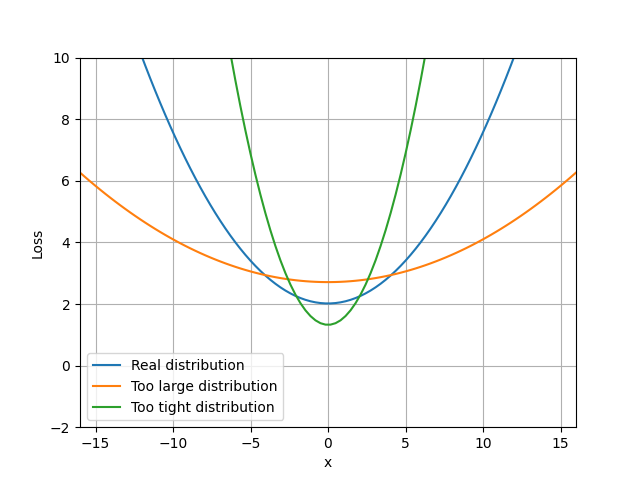
\includegraphics[width=400px]{distribution_comp.png}
    \caption{Comparison of the loss for a perfectly predicted distribution, a too large predicted distribution and a too tight distribution, with x the difference between the observed value and the median of the predicted distribution}
    \label{fig:distrib_comp}
\end{figure}


\subsection{Metrics} \label{metrics}

Concerning the evaluation of the results, GluonTS provides a module using the trained model and testing data to provide quantitative results, as metrics ("Aggregate", for all time series, or "Item", for each series separately). Metrics proposed by GluonTS includes \textit{MSE, MSIS, RMSE}, and other classical measures.

All metric function takes as argument \textit{N} randomly drawn sample values of the predicted probability distribution ($[{x_1},...,{x_N}]$) and one observed value y. 
For example the MSE metric function is defined as :
\begin{equation}
    MSE(y,[{x_1},...,{x_N}]) = \frac{1}{N}\sum_{i=0}^{N}(y-{x_i})^2
\end{equation}

"Item" metric value is the mean of metric value for each time step of the prediction window.
"Aggregate" metric value is the mean of "Item" metrics values for each time series.

In chapter \ref{part3}, as we use the default loss, metric function must correspond to this loss function, as it has been defined in section \ref{loss}. 

The problem is that the metric function cannot be equivalent to loss function, as these are functions with different inputs, the loss function taking as input the predicted distribution instead of randomly drawn point sample.
Nowadays, in fine, metrics like \textit{MSE, MSIS, RMSE} expresses the same goal than the log-negative likelihood of the loss function, i.e. the minimization of the difference between predicted and real distribution.
A high value of one of these metrics is proportional to a high value of the loss.
The metric chosen for the first model comparison in chapter \ref{part3} is \textit{MSE}.



\subsection{Distribution}\label{distribution}

GluonTs proposes different types of output distribution. In most of the models the output is technically
 a vector of values which is
transformed to a vector of distribution parameters  and put in a distribution object.
In current implementation, three different output distribution are functional. $Gaussian$, $Laplace$ and $PiecewiseLinear$.
$Student$ has been rejected because the quantiles of the distribution are not obtainable.
$Uniform$ has been rejected because of loss problems in execution.
Other options are available, as multiple kernel gaussian.
The GluonTS models are mandatory to output an object containing point sample of the distribution, not the distribution itself (parameters values). Considering that the parameter information could also be useful, as asked by the client, a modification done in custom models allows saving these information.

\begin{figure}[H]
    \centering
    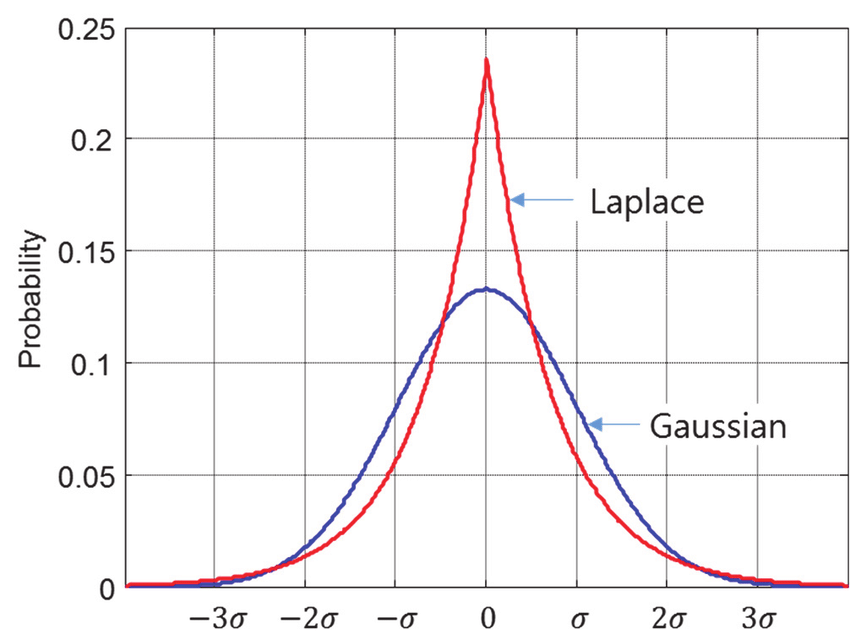
\includegraphics[width=200px]{Gaussian-distribution-and-Laplace-distribution.ppm.png}
    \caption{Comparison between Gaussian distribution and Laplace distribution}
    \label{fig:gausslaplace}
\end{figure}

\begin{figure}[H]
    \centering
    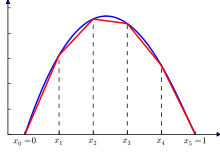
\includegraphics[width=200px]{220px-Finite_element_method_1D_illustration1.svg.png}
    \caption{Comparison between Gaussian distribution and PiecewiseLinear distribution}
    \label{fig:gausslaplace}
\end{figure}

\subsection{Models presentation} \label{diff_models}


All the pre-implemented deep learning models that have been tested  are presented here.
The models individual hyperparameters are mentioned in corresponding section.
The results for different values of hyperparameters are studied in section \ref{comp_model_param}.


\subsubsection{Simple} \label{descr_simple}
A manually implemented model which uses a simple 2 fully connected layers neural network.
The individual hyperparameter is the number of cells in layers.

\subsubsection{FeedForward} \label{descr_feedfordward}
A MLP (multi-layer perceptron) model.
The individual hyperparameter is the number of hidden nodes in each layer.

\subsubsection{Recurrent Neural Network} \label{descr_canonicalRNN}
A model which uses a recurrent neural network \ref{rnn_paper}.
The individual hyperparameters are the number of layers and number of cells of the network

\subsubsection{DeepAr} \label{descr_deepar}
Implementation of DeepAr estimator, a RNN based model, close to the one described in paper 
\textit{"DeepAR: Probabilistic Forecasting with Autoregressive Recurrent Networks"} \cite{deepar_paper}.
The individual hyperparameters are the same than for CanonicalRNN.

\subsubsection{Deep Factors} \label{descr_deepfactor}
Implementation of the 2019 ICML paper \textit{“Deep Factors for Forecasting”} \cite{deepar_factor}.
Uses a global RNN model to learn patterns across multiple related time series and an arbitrary local model to model the time series on a per time series basis. 
In the current implementation, the local model is a RNN (DF-RNN).
The individual hyperparameters are the number of units per hidden layers and the number of layers in the global model, the number of units and layers in the local model (not studied)
, the number of global factors.

\subsubsection{Gaussian Process} \label{descr_gp}
Model using Gaussian Processes (GP) \cite{gp_paper}.
Each time series has a GP with its own hyper parameters.
There are no hyperparameters to tune.

\subsubsection{NPTS} \label{descr_npts}
Implementation of the Non-Parametric Time Series Forecaster \cite{npts_paper}, 
which falls into the class of simple forecasters that use one of the past observed targets as the forecast for
the current time step. It randomly samples a past time index as the prediction for the time step T (auto regressive model, which predict step by step).
There are no hyperparameters to tune, but it exists some variants.

\subsubsection{MQCNN} \label{descr_mqcnn}
Discriminative Sequence to Sequence model constructed using the \textit{SeqtoSeq} framework of GluonTS to reproduce the model of the 
paper \textit{"A Multi-Horizon Quantile Recurrent Forecaster"}\cite{mqcnn_paper}.
Sequence to sequence models are composed of two parts. The encoder network, that reads the training window of the time series 
and encodes information about  the  sequence  in  a  latent  state.
And the decoder network, which generates the forecast by combining the latent information with the features in the prediction range.
In MQCNN, the encoder is a Convolutionnal Neural Network and the decoder an MLP. Unlike other presented models, the output is not technically a distribution but the quantiles itself, that are point predicted values obtains by optimizing the corresponding quantile loss.
The individual hyperparameter is the  dimension of the MLP decoder.
Considering the fundamental difference in the intern functioning, it not seems to be possible to modify the loss, see discussion in \ref{custom_loss} section.

\subsubsection{MQRNN} \label{descr_mqrnn}
Same as MQCNN but with a Recurrent Neural Network encoder instead.

\subsection{Others}

Other models, recently added to GluonTS,  will be added. At least 3 (Wavenet, DeepVar, NBEATS)
